\chapter{Shranjevanje delotokov}
\label{ch:shranjevanje-delotokov}

Če ste do sedaj sledili vsem navodilom - razen tistih seveda, kjer smo odstranjevali gradnike - potem vaš delotok izgleda nekako takole.\marginnote{Še en trik: Ctrl-C (oz. or Cmd-C na Mac OS) prekopira vizualizacijo na odložišče (npr. iz Scatter Plota), od koder jo lahko s Ctrl-V (Cmd-V ) prenesete v drugo aplikacijo (npr. Word).}

\begin{figure}[h]
    \centering
    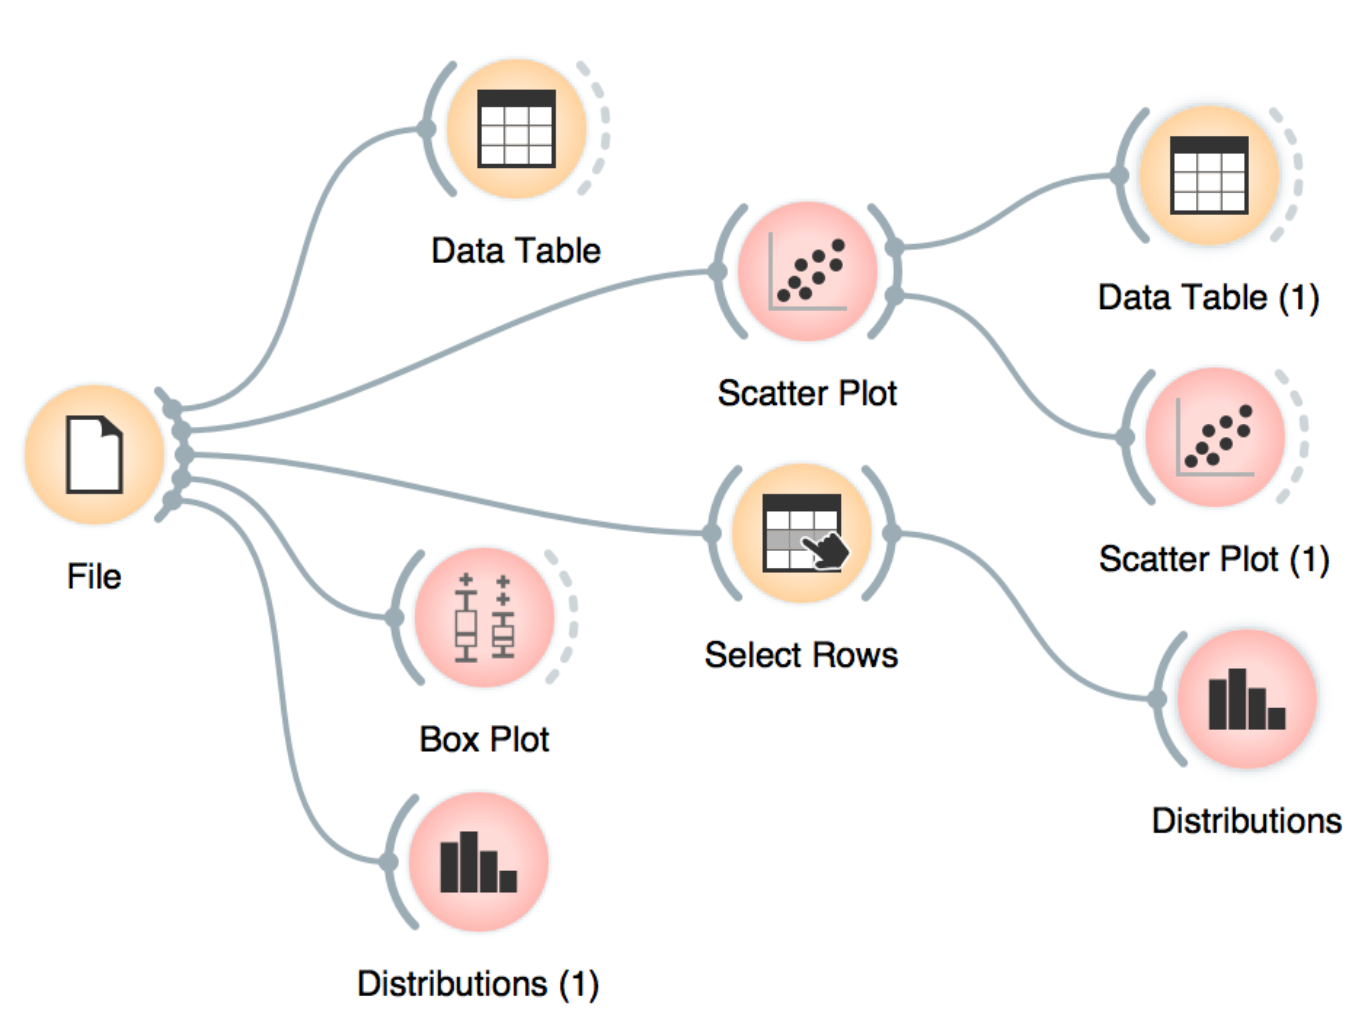
\includegraphics[width=0.9\linewidth]{workflow.png}%
    \caption{$\;$}
    \label{fig:workflow}
  \end{figure}

Delotok lahko shranite (File $\rightarrow$ Save) in ga delite s sodelavci. Vendar pa morate v isti direktorij priložiti tudi podatke, sicer bo Orange naložil zgolj shemo.

\begin{figure*}[h]
    \centering
    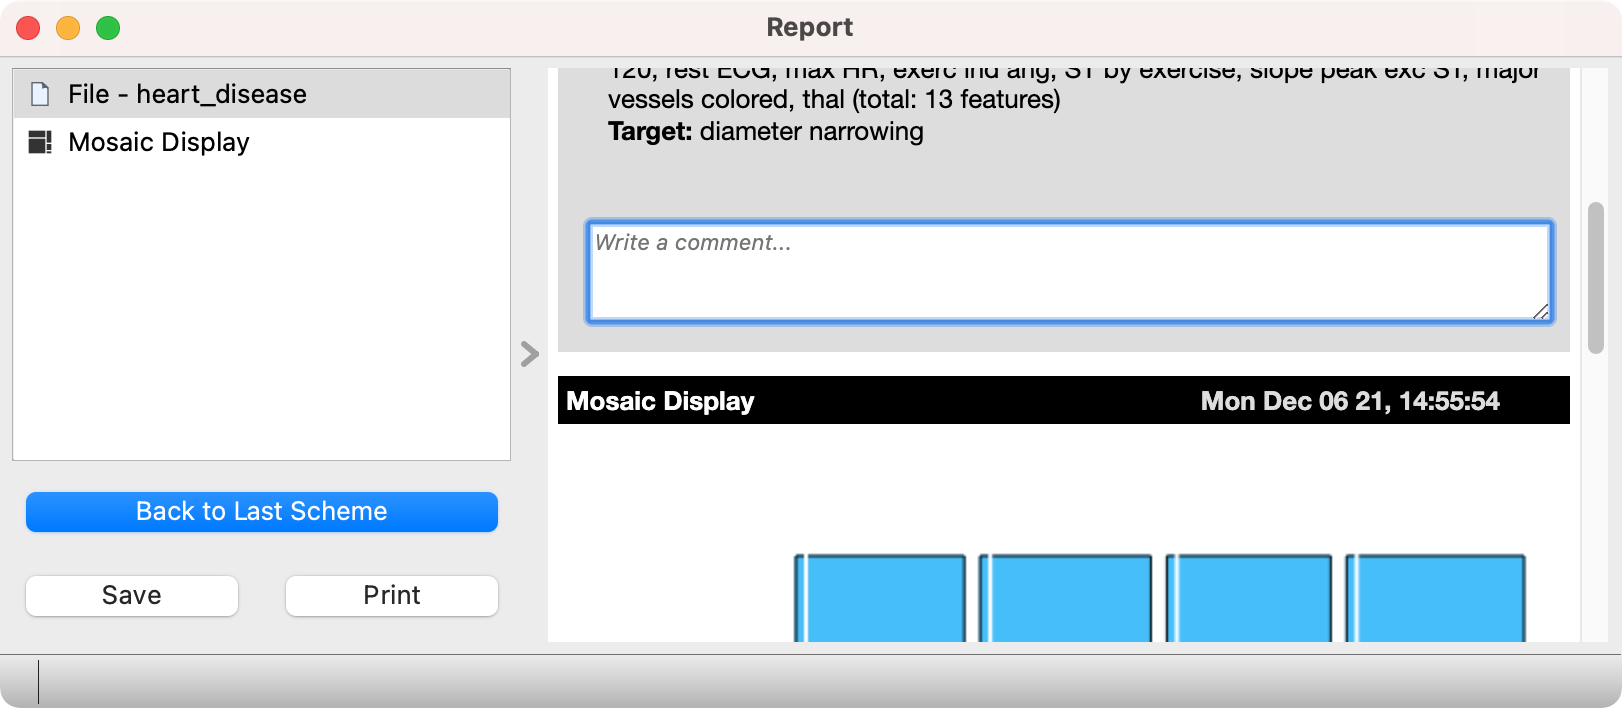
\includegraphics[width=0.9\linewidth]{report-full.png}%
    \caption{$\;$}
    \label{fig:report-full}
  \end{figure*}

\newpage

Gradniki imajo na dnu okna orodno vrstico. Tam lahko odpremo pomoč (opis uporabe gradnika), shranimo vizualizacijo in dodamo gradnik v poročilo.

\begin{marginfigure}
    \centering
    
\includegraphics[width=40mm]{status-bar2.png}
    \caption{Orodna vrstica. Po vrsti si sledijo možnosti za pomoč, shranjevanje grafov in poročilo. V drugem delu vrstice so vhodi v gradnik in izhodi iz njega.}
    \label{fig:status-bar2}
\end{marginfigure}

\begin{figure}[h]
    \centering
    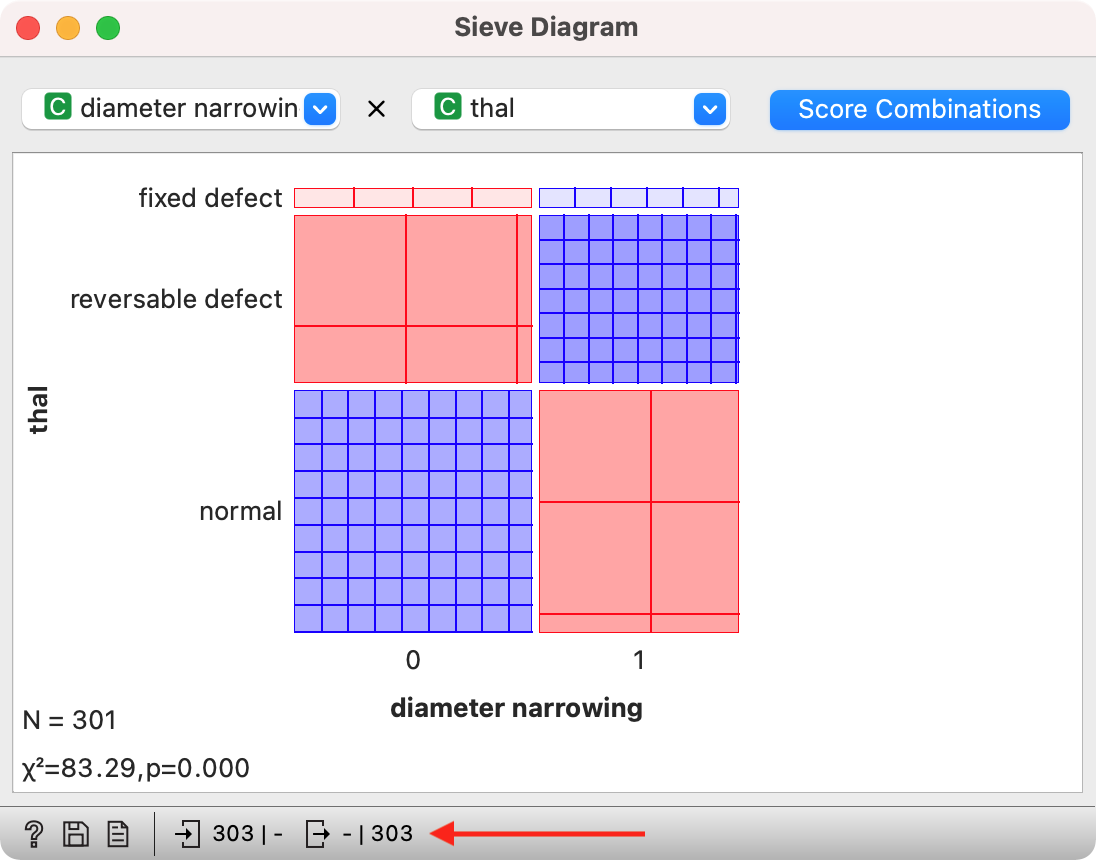
\includegraphics[width=\linewidth]{status-bar.png}%
    \caption{$\;$}
    \label{fig:status-bar}
\end{figure}

Ko odkrijete kaj zanimivega v gradniku, kot je npr. nepričakovani Sievov diagram za paciente, kliknite \textit{Report}. S tem dodate vizualizacijo v poročilo. V poročila lahko vnesemo vse gradnike, ki vodijo do zanimivega odkritja, saj tako natačno vemo, kako smo prišli do rezultatov.

Vsak del poročila omogoča tudi dodajanje komentarjev.

\begin{figure}[h]
    \centering
    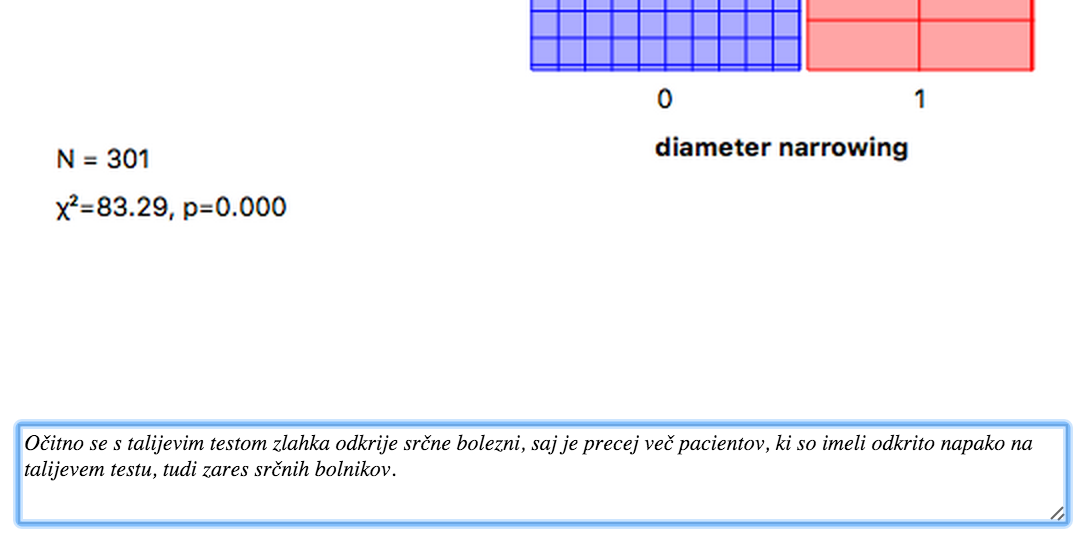
\includegraphics[width=\linewidth]{report-comment.png}%
    \caption{$\;$}
    \label{fig:report-comment}
\end{figure}

Poročila lahko shranjujete v formatu HTML ali PDF ali pa kot datoteko, ki shrani vse delotoke, povezane z vizualizacijo. Te lahko kasneje tudi odprete in pregledate v Orangeu. Tako lahko vi in sodelavci enostavno ponovite analizo.
